\documentclass[a4paper, notitlepage]{article}
\usepackage[all]{xy}
\usepackage[final]{pdfpages}
\usepackage{verbatim}

%\renewcommand{\item[]}{\textbf{}}
\newcommand{\boldItem}[1]{\item[\textbf{#1}]}

\title{Draft Workplan}
\author{Wadie Assal \\ 6398693 \and Jeroen Rooijmans \\ 5887410 \and Jasper Timmer \\ 5995140 \and Maarten de Waard \\ 5894883 \and Maarten Inja (vz) \\ 5872464}

\begin{document}

\maketitle


\section{Specification}
In this chapter you can find a list of the products that will be delivered
during the project Software Engineering and Distributed Applications (BINSEGA6). You can also find a description of the product and witch specifications it will comply to. 

\subsection{Work plan}
The work plan is the document you are reading now. The work plan will contain
design decisions, the project planning and specifications of the different
software components. Furthermore it will contain the information needed to start
the project. It will also function as guidance during the project. 

\subsection{Presentation}
We are going to present our finished software product on Thursday in week 26.
This will be done with the help of a slide show. The following subjects
are going to be discussed in this presentation:
\begin{itemize}
\item How did the development process go?
\item What can the software product do?
\item What can’t the software product do?
\item What can be improved in future?
\end{itemize}

\subsection{Demonstration}
The demonstration is going to be given right after the presentation mentioned
above. The sole purpose of the demonstration is showing that our software works
correctly as specified in the delivered documents. We will be proving this by
running our software in different scenarios.

\subsection{Final report}
The final report is going to be the last delivered product. After a review with
the professor of the draft, we will use the given feedback to produce the final version of this product. You can find the following subjects 
in the final report: 
\begin{itemize}
\item Project goals
\item The development process
\item Software architecture and explanation of design decisions
\item Software manual
\end{itemize}

\subsection{AP2DX Software}
This is the actual software that has to be delivered. The goal of the software
is to use a robot to map an area. During the mapping the robot needs to avoid
obstacles and he has to constantly know where he is on the map. Further
requirements are:
\begin{itemize}
\item The software needs to be distributed
\item Limited failsafe possibilities
\item It should run over a network or on one device
\end{itemize}



\section{Functionial Design}
\begin{figure}
\centering
\xymatrix{& USARSim \ar@/_/[d] &  \\
& Coordinator \ar@/_/[u] \ar[dr] & \\
Abstract Motor \ar[ur] & Reflex \ar[l]  & Sensor \ar[l] \ar[d] \\
& Planner \ar[u] & Mapper \ar[l] }
\caption{A representation of our functional design}
\label{fig:fd}
\end{figure}

\subsection{Components}
This section will discuss the components of the functional design seen in figure
\ref{fig:fd}
\subsubsection{Coordinator}
This module will coordinate data traffic between the USARSim engine and
our program. It distributes the data to several modules, as can be
seen in the diagram.
\subsubsection{Abstract Motor}
With this module, we maneuver the P2DX robot in the virtual world. We
can control two motors, one connected to the left wheel and one to the
right wheel. When a path is planned or a reflex kicks in, it sends a
command to the Abstract Motor module. This translate the given
commando to a series of operations we then apply to the virtual motors.
\subsubsection{Sensor}
The sensor module collects sensory data from the robot. This data is
checked and translated. If certain data crosses a critical level, a
command is sent to Reflex to prevent the robot from crashing. All
data is translated and sent to our Mapper.
\subsubsection{Reflex}
To prevent the robot from crashing, we implement a module that is
always checking the sensory data. When some critical level is reached (e.g. a
wall gets too close in front of our robot, or the motors try to turn, but the
wheels do not) we take action, thus preventing our robot from breaking. 
\subsubsection{Mapper}
To be able to plan routes and navigate through the environment, our robot should
be able to create a map. This map is a representation of its environment, based
on the sensory data the robot receives. This module will also be able to track
the robots location in this map, by using data from, for example, the wheel
sensors.
\subsubsection{Planner}
To be able to create a map, our robot
needs to plan a path to (and through) unknown regions. Our planner sends the
robot to new areas, while avoiding obstacles. The Planner also
calculates our current location in the environment and checks if our
location is on the path we want to follow. The Planner uses data from
the Sensor and from the Mapper.

\section{Milestones}
This section will describe the milestones, and what deliverables we will provide. 

\subsection*{Milestone 0}
This will describe what we will have done by the 10th of June. These are the
deliverables:
\begin{description}
\vspace{0cm}
\item[Working environment:] We will set up a Git
repository\footnote{https://github.com/Y3PP3R/AP2DX} and a testing environment
(using jUnit).
\item[Base class:] We will make an abstract base class, on which we can base
all our Java classes. This will contain all the standard methods, e.g. TCP/IP
protocols.
\end{description}

\subsection*{Milestone 1}
This will describe which deliverables we will have done by the 
\begin{description}
\item[Drive:] We want the program to be able to direct
the robot through the environment. We will not yet focus on the ability to
follow lines or walls.
\item[Avoid collision:] The robot should be able to avoid collision with objects
and walls. It will stop, turn a random corner, and drive on. This way it will
cover most of the area without colliding.
\end{description}

Classes needed to be implemented for these goals:
\begin{itemize}
\item Co\"ordinator
\item Sensor
\item Reflexes
\item Motor
\end{itemize}

\subsection*{Milestone 2}
A list of deliverables:
\begin{description}
\item[Avoid obstacles:] The robot will be able to avoid the obstacles that
cross his path, in stead of stopping and turning a random corner.
\item[Navigate:] The robot will be able to navigate through the room.
\end{description}

What we will implement for this:
\begin{description}
\item[Mapper:] A class that creates a map of the room out of the sensor
data. In the time of milestone 2 it does not have to be able to create an entire
map and be very accurate, but it will be able to make some implementation.
\item[Improved Sensor:] The sensor class will be improved to be able to make
an accurate map.
\item[Improved Reflexes:] The reflex class needs to be able to use some
sensor data to be able to avoid objects appropriately. 
\end{description}


\subsection*{Demonstration}
Before the demonstration we will be able to do the following things:
\begin{description}
\item[Planner:] We will have a planner class that can specify directions
based on the current map position and what part of the map we have not yet
discovered.
\item[Improved Mapper:] The mapper will now be able to make an accurate map
and find our location on it, while taking the errors in sensor data into account.
\item[Tests:] Although we test all the time, we want to have tested
everything good before the end.
\item[Report:] We will work on a report, describing our progress, problems
and (test)results.
\item[Documentation:] We will work on a proper documentation of our code,
which is also finished before the end.
\end{description}

The classes we will need to implement or improve for this are:
\begin{itemize}
\item Mapper
\item Planner
\item All test classes
\end{itemize}

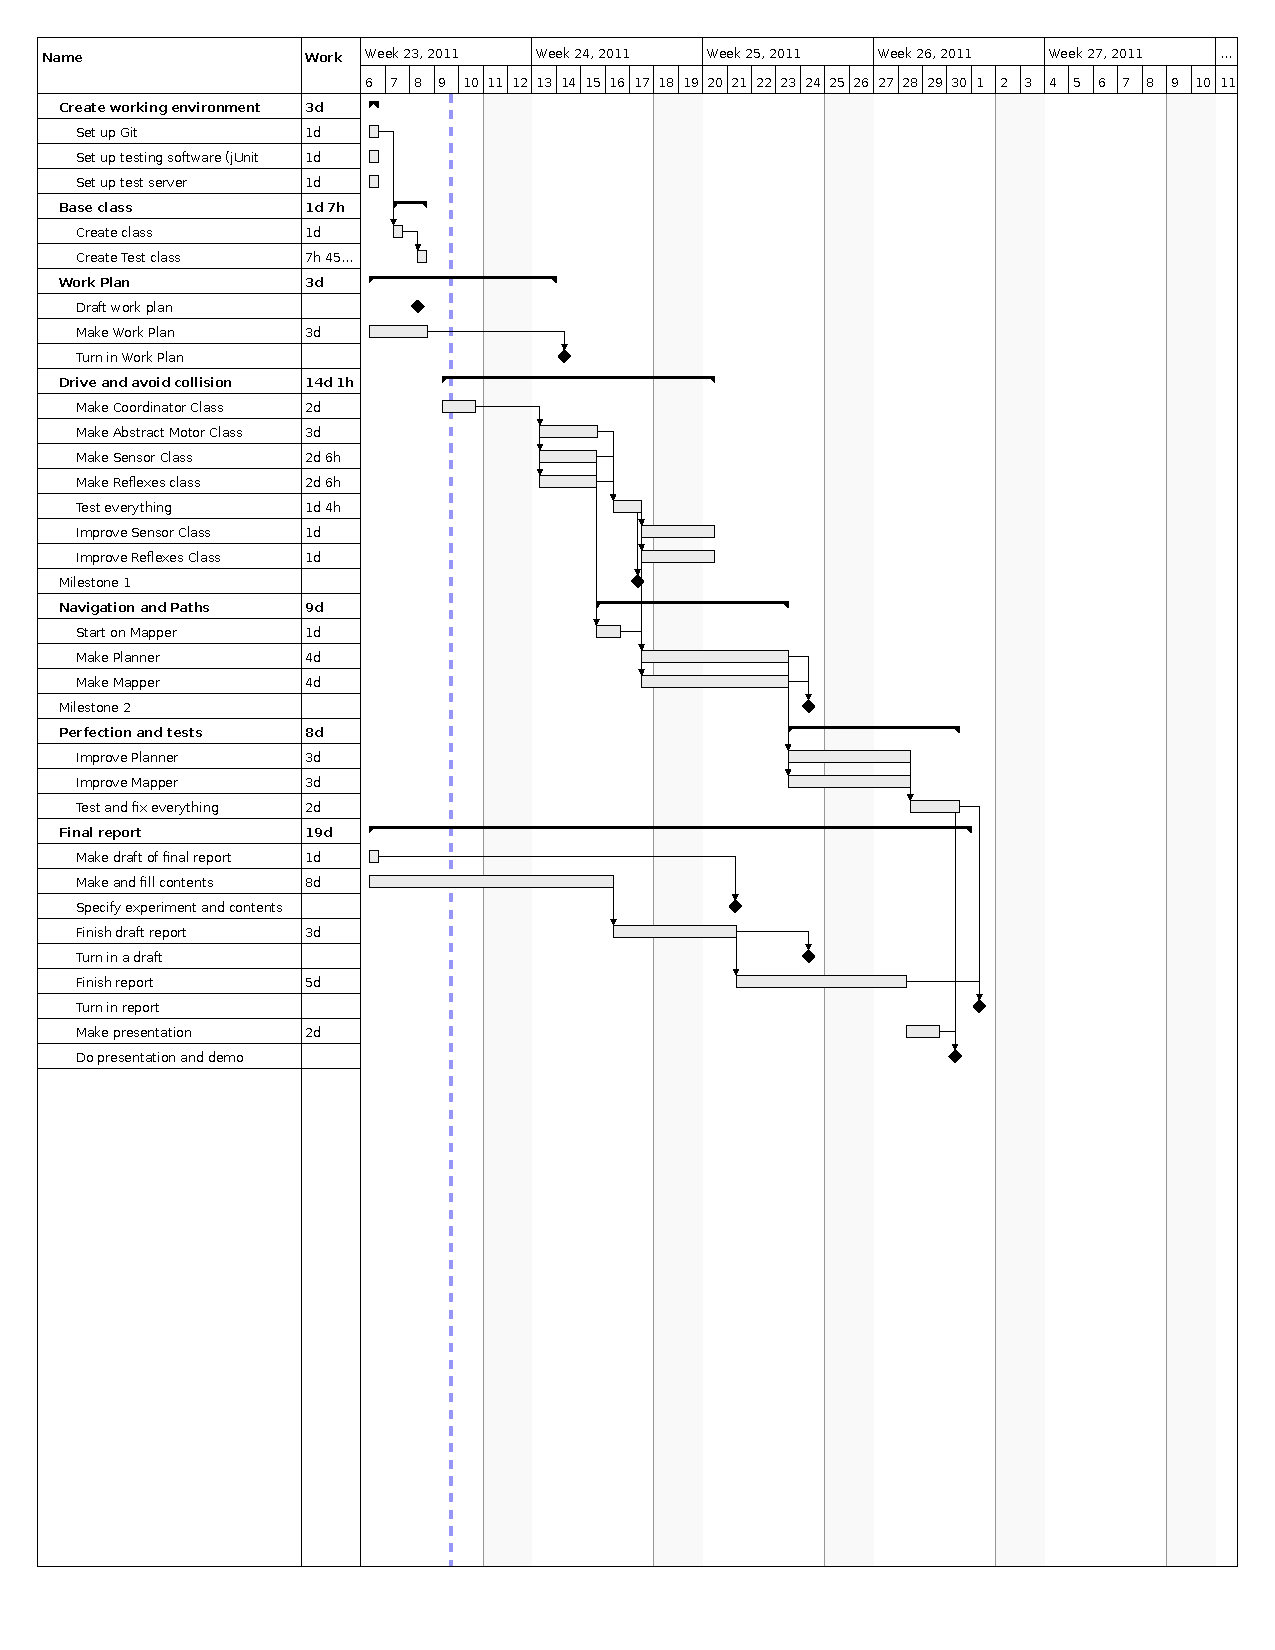
\includepdf{planner}
\end{document}
